\documentclass{article}
\usepackage{amsmath}
\usepackage{amssymb}
\usepackage{amsthm}
\usepackage{enumitem}
\usepackage{graphicx}
\usepackage{tcolorbox}
\tcbuselibrary{theorems}
\tcbuselibrary{breakable}

\newtcbtheorem[number within=section]{mythm}{Theorem}%
{colback=green!5,colframe=green!35!black,fonttitle=\bfseries,breakable}{th}
\newtcbtheorem[use counter from=mythm]{mydef}{Definition}%
{colback=blue!5,colframe=blue!35!black,fonttitle=\bfseries,breakable}{de}
\newtcbtheorem[use counter from=mythm]{myrem}{Remark}%
{colback=white!5,colframe=white!35!black,fonttitle=\bfseries,breakable}{re}
\newtcbtheorem[use counter from=mythm]{myex}{Example}%
{colback=orange!5,colframe=orange!35!black,fonttitle=\bfseries,breakable}{ex}
\newtcbtheorem[use counter from=mythm]{myprop}{Proposition}%
{colback=green!5,colframe=green!35!black,fonttitle=\bfseries,breakable}{pr}

\setcounter{tocdepth}{2}
\setlength\parindent{0pt}
\hyphenpenalty 10000

\title{STAT 240 Course Notes - Fall 2018}
\author{Max Zhu}

\begin{document}
	\maketitle\newpage
	\tableofcontents\newpage
	
	\section{Foundations}
	Andrey Kolmogorov \textit{(1933, ``Foundations of the theory of probability")} put probability on solid mathematical grounds using a model, probability space $(\Omega, \mathcal{F}, P)$. A probability space consists of:
	\begin{enumerate}
		\item Sample space $\Omega$: set of all outcomes $\omega$
		\item $\sigma$-algebra $\mathcal{F}$: set of all events, i.e. subsets of $\Omega$ to which we can assign a probability
		\item Probability measure $P: \mathcal{F} \rightarrow  [0, 1]$: function which assigns probabilities to events
	\end{enumerate}
	
	We need measure theory to understand this.
	
	\subsection{$\sigma$-algebras and measures}
	A classical problem is to measure the volume $\lambda(A)$ of some $A\subseteq \mathbb{R}^d, d\geq 1$. Consider $d=1$. Then, $\lambda$ should:
	\begin{enumerate}[label=(\roman*)]
		\item Assign to intervals its length: $\lambda([a, b])=b-a$ for all $a, b\in \mathbb{R}, a \leq b$
		\item Be invariant under translations, rotations, and reflections: $\lambda(A)=\lambda(B)$ for all congruent $A, B\subseteq \mathbb{R}$
		\item Be $\sigma$-additive:\\
		If $\{A_i\}_{i\in\mathbb{N}}\subseteq\mathbb{R}, A_i\cap A_j=\varnothing\;\forall i\neq j$, then $\lambda(\bigcup_{i=1}^{\infty}A_i)=\sum_{i=1}^{\infty}\lambda(A_i)$\\\\
		In other words, the volume of the union of countably many subsets of $\mathbb{R}$ is equal to the sum of their volumes.
	\end{enumerate}
	
	Can we take the power set $\mathcal{P}(\mathbb{R})=\{A : A\subseteq \mathbb{R}\}$ as $\mathcal{F}$ and find such a $\lambda$?
	
	\begin{mythm}{Vitali's Theorem}{}
		There exists no $\lambda$ defined on $\mathcal{P}(\mathbb{R})$ which fulfils (i)-(iii). Any measurable set $A\subseteq\mathbb{R}: \lambda(A)>0$ contains a non-measurable set $V$ (Vitali set). 
	\end{mythm}
	
	What about weakening (iii) to finitely many sets? Still no!
	
	\begin{mythm}{Banach-Tarski}{}
		Let $d\geq 3$ and $A, B\in \mathbb{R}^d$ be bounded with non-empty interior. Then, there exists $k\in\mathbb{N}$ and partitions:
		\begin{align*}
			A=\dot\bigcup_{i=1}^kA_i\\
			B=\dot\bigcup_{i=1}^kB_i
		\end{align*}
		such that $A_i, B_i$ are congruent $\forall i\in \{1,..., k\}$.
	\end{mythm}
	
	For countable $\Omega$, one can define $\lambda$ (or $\mu$ or $P$) on $\mathcal{P}(\Omega)$ but for uncountable $\Omega$, $\mathcal{P}(\Omega)$ is too large. Therefore, we need to define $\lambda, \mu, P$ on some proper subset of $\mathcal{P}(\Omega)$ which is closed under certain set operations.
	
	\begin{mydef}{$\sigma$-algebra}{}
		$\mathcal{F}\subseteq\mathcal{P}(\Omega)$ is a \underline{$\sigma$-algebra} on $\Omega$ if:
		\begin{enumerate}[label=(\roman*)]
			\item $\Omega\in\mathcal{F}$
			\item $A\in\mathcal{F}\Rightarrow A^c\in\mathcal{F}$
			\item $\{A_i\}_{i\in\mathbb{N}}\subseteq\mathcal{F}\Rightarrow\bigcup_{i=1}^{\infty}A_i\in\mathcal{F}$
		\end{enumerate}
		If (iii) holds for only finitely many sets, $\mathcal{F}$ is an \underline{algebra}.
	\end{mydef}
	
	\begin{myrem}{}{}
		$\sigma$-algebras are closed w.r.t. countable intersection, since
		\begin{equation*}
			\bigcap_{i=1}^{\infty}A_i=(\bigcup_{i=1}^{\infty}A_i^c)^c\in\mathcal{F}
		\end{equation*}
		by de Morgan.
	\end{myrem}
	
	\begin{myex}{}{}
		\begin{enumerate}
			\item Trivial $\sigma$-algebra: $\{\varnothing, \Omega\}=\mathcal{F}$
			\item $\mathcal{F}=\{\dot\bigcup_{i=1}^n(a_i, b_i] : 0\leq a_i\leq b_i\leq 1\;\forall i, n\in\mathbb{N}\}$ is an algebra on $\Omega=(0, 1]$ but not a $\sigma$-algebra since $\dot\bigcup_{n=0}^{\infty}(\sum_{k=1}^{2n}(\frac{1}{2})^k, \sum_{k=1}^{2n+1}(\frac{1}{2})^k]\notin\mathcal{F}$, while $(\sum_{k=1}^{2n}(\frac{1}{2})^k, \sum_{k=1}^{2n+1}(\frac{1}{2})^k]\in\mathcal{F}$ for all $k$.
		\end{enumerate}
	\end{myex}
	
	How can $\sigma$-algebras be constructed?
	
	\begin{myprop}{}{}
		Given $A\subseteq\mathcal{P}(\Omega)$, then there exists a unique minimal $\sigma$-algebra $\sigma(A)$ which contains all sets of $A$: a $\sigma$-algebra generated by A. $\sigma(A)$ is the intersection of all $\sigma$-algebras of which A is a subset.
		
		\begin{proof}
		Let $\mathcal{F}_A=\{\mathcal{F} : \mathcal{F}$ is a $\sigma$-algebra, $A\subseteq\mathcal{F}\}$. Then, $\sigma(A)$ is a $\sigma$-algebra since:
		\begin{enumerate}[label=(\roman*)]
			\item $\Omega\in\mathcal{F}\;\forall\mathcal{F}\in\mathcal{F}_A$ since all $\mathcal{F}\in\mathcal{F}_a$ is a $\sigma$-algebra
			\item $A\in\sigma(A)\Rightarrow A\in\mathcal{F}\;\forall\mathcal{F}\in\mathcal{F}_A\Rightarrow A^c\in\mathcal{F}\;\forall\mathcal{F}\in\mathcal{F}_A\Rightarrow A^c\in\sigma(A)$.
			\item If $\{A_i\}_{i\in\mathbb{N}}\subseteq \sigma(A)$, then $\{A_i\}_{i\in\mathbb{N}}\subseteq\mathcal{F}\;\forall\mathcal{F}\in\mathcal{F}_A$.\\ So, $\bigcup_{i=1}^{\infty}A_i\in\mathcal{F}\;\forall\mathcal{F}\in\mathcal{F}_A$, so $\bigcup_{i=1}^{\infty}A_i\in\sigma(A)$.
		\end{enumerate}
		
		So $\sigma(A)$ is a $\sigma$-algebra. Now, $\sigma(A)\supseteq A$ since $\mathcal{F}\supseteq A\;\forall\mathcal{F}\in\mathcal{F}_A$. Also, $\forall\;\sigma$-algebra $\mathcal{F}'\supset A$, we have $\mathcal{F}'\in\mathcal{F}_A$, so $\mathcal{F}'\supseteq\sigma(A)$.\\
		
		Therefore, $\sigma(A)$ is the minimal $\sigma$-algebra containing A.
	\end{proof}
	\end{myprop}
	
	\begin{myrem}{}{}
		Unless $|\Omega|<\infty$, a construction of $\sigma(A)$ is typically hopeless.
	\end{myrem}
	
	\begin{myex}{}{}
		$\mathcal{B}(\Omega):=\sigma(\{O : O\subseteq\Omega, O$ is open$\})$ is the Borel $\sigma$-algebra on $\Omega$. Its elements are called Borel sets. For $\Omega=\mathbb{R}^d$ one can show that
		\begin{align*}
			\mathcal{B}(\mathbb{R}^d)&=\sigma(\{(a, b] : a\leq b\})\\
			&=\sigma(\{(a, b) : a\leq b\})\\
			&=\sigma(\{[a, b] : a\leq b\})\\
			&=\sigma(\{(-\infty, b]\})
		\end{align*}
		and so on. Borel sets contain open sets, closed sets, and countable union and intersections of these sets.
	\end{myex}
	
	\begin{mydef}{}{}
			Let $\mathcal{F}$ be a $\sigma$-algebra on $\Omega$. Then, $(\Omega, \mathcal{F})$ is a \underline{measurable space}, sets in $\mathcal{F}$ are \underline{measurable sets}. A \underline{measure} $\mu$ on $\mathcal{F}$ is a function such that:
			\begin{enumerate}[label=(\roman*)]
				\item $\mu : \mathcal{F}\rightarrow [0, \infty]$
				\item $\mu(\varnothing)=0$
				\item Let $\{A_i\}_{i\in\mathbb{N}}\subseteq\mathcal{F}, A_i\cap A_j=\varnothing\;\forall i\neq j$. Then, $\mu(\dot\bigcup_{i=1}^{\infty}A_i)=\sum_{i=1}^{\infty}\mu(A_i)$. ($\sigma$-additivity)
			\end{enumerate}
			
			$(\Omega, \mathcal{F}, \mu)$ is then called a \underline{measure space}.\\
			
			If $\Omega=\bigcup_{i=1}^{\infty}A_i$ for $\{A_i\}_{i\in\mathbb{N}}\subseteq\mathcal{F}: \mu(A_i)<\infty\;\forall i$, then $\mu$ is \underline{$\sigma$-finite}.\\
			
			If $\mu(\Omega)<\infty$, $\mu$ is a \underline{finite measure}.\\
			
			A measure $\mu$ on $\mathcal{B}(\mathbb{R}^d)$ is a \underline{Borel measure} on $\mathbb{R}^d$.
	\end{mydef}
	
	\begin{myrem}{}{}
		\begin{enumerate}
			\item $\sigma$-additivity (in contrast to finite additivity) allows for limiting processes (pointwise limits of "measurable functions" are measurable). Many fundamental consequences follow, such as Central Limit Theorem and Law of Large Numbers.
			\item Uncountable additivity is too strong, since for any $A\subseteq \mathbb{R}$:
			\begin{align*}
				\lambda(A)&=\lambda(\bigcup_{x\in A}\{x\})\\
				&=\sum_{x\in A}\lambda(\{x\})\\
				&=sup_{A'\subseteq A, |A'|<\infty}\sum_{x\in A}\lambda(\{x\})\\
				&=0
			\end{align*}
		\end{enumerate}
	\end{myrem}
	
	\begin{myex}{}{}
		If $\Omega$ is countable, $\mathcal{F}=\mathcal{P}(\Omega)$, $\forall f : \Omega\rightarrow[0, \infty]$, $\mu(A)=\sum_{\omega\in A}f(\omega)\;\forall A\in\mathcal{F}$ defines a measure on $\mathcal{F}$.\\
		
		If $f(x)=1\;\forall x\in\Omega$, $\mu$ is called a counting measure.\\
		
		Suppose for some $\omega_0\in\Omega, f(\omega)=1$ if $\omega=\omega_0$, $0$ otherwise. Then $\mu$ is point mass or Dirac measure.
	\end{myex}
	
	\begin{myprop}{}{}
		Let $(\Omega, \mathcal{F}, \mu)$ be a measure space. Then:
		\begin{enumerate}
			\item $A, B\in\mathcal{F}, A\subseteq B\Rightarrow\mu(\bigcup_{i=1}^{\infty}A_i)\leq\sum_{i=1}^{\infty}\mu(A_i)$ (monotonicity)
			\item $\{A_i\}_{i\in\mathbb{N}}\subseteq\mathcal{F}\Rightarrow\mu(\bigcup_{i=1}^{\infty}A_i)\leq\sum_{i=1}^{\infty}\mu(A_i)$ (sub additivity)
			\item \begin{align*}
				\{A_i\}_{i\in\mathbb{N}}\subseteq\mathcal{F}, A_1\subseteq...\subseteq A_n\subseteq...\Rightarrow\mu(\bigcup_{i=1}^{\infty}A_i)&=\mu(\lim_{n\to\infty}\bigcup_{i=1}^{n}A_i)\\
				&=\lim_{n\to\infty}\mu(A_n)
			\end{align*}
			(continuity from below)
			\item \begin{align*}
				\{A_i\}_{i\in\mathbb{N}}\subseteq\mathcal{F}, A_1\supseteq...\supseteq A_n\supseteq...\Rightarrow\mu(\bigcap_{i=1}^{\infty}A_i)&=\mu(\lim_{n\to\infty}\bigcap_{i=1}^{n}A_i)\\
				&=\lim_{n\to\infty}\mu(A_n)
			\end{align*} for $\mu(A_1)<\infty$.
			(continuity from above)
		\end{enumerate}
		
		\begin{proof}~\\
		\begin{enumerate}
			\item $B=A\dot\cup(B\backslash A)$\\
			Therefore, $\mu(B)=\mu(A)+\mu(B\backslash A)\geq0$\\
			$\mu(B)\geq\mu(A)$ and if $\mu(A)<\infty$,\\
			$\mu(B\backslash A)=\mu(B)-\mu(A)$.
			\item Let $B_1=A_1$, $B_n=A_n\backslash \bigcup_{i=1}^{n-1}A_i\subseteq A_n\;\forall n\geq2$.\\
			So, all $B_n$ are pairwise disjoint and $\bigcup_{i=1}^{n}B_i=\bigcup_{i=1}^{n}A_i\;\forall n\in\mathbb{N}$.\\
			So, $\mu(\bigcup_{i=1}^{\infty}A_i)=\mu(\bigcup_{i=1}^{\infty}B_i)=\sum_{i=1}^{\infty}\mu(B_i)\leq\sum_{i=1}^{\infty}\mu(A_i)$.
			\item Let $A_0=\varnothing$. Then,
			\begin{align*}
				\mu(\bigcup_{i=1}^{\infty}A_i)&=\mu(\bigcup_{i=1}^{\infty}(A_i\backslash A_{i-1})\\
				&=\sum_{i=1}^{\infty}\mu(A_i\backslash A_{i-1})\\
				&=\lim_{n\to\infty}\sum_{i=1}^{n}\mu(A_i\backslash A_{i-1})\\
				&=\lim_{n\to\infty}\mu(A_n)
			\end{align*}
			\item Let $B_i=A_1\backslash A_i=A_1\cap A_i^c\;\forall i\in\mathbb{N}$. Then, $B_1\subseteq B_2\subseteq...$
			\begin{align*}
				\bigcup_{i=1}^{\infty}B_i&=\bigcup_{i=1}^{\infty}(A_1\cap A_i^c)\\
				&=A_1\cap\bigcup_{i=1}^{\infty}A_i^c\\
				&=A_1\cap(\bigcap_{i=1}^{\infty}A_i)^c\\
				&=A_1\backslash\bigcap_{i=1}^{\infty}A_i
			\end{align*}
			!!!
		\end{enumerate}
	\end{proof}
	\end{myprop}
	
	\subsection{Probability Measures}
	
	\begin{mydef}{}{}
		Let $(\Omega, \mathcal{F})$ be a measure space. Then, a \underline{probability measure} $P$ on $\mathcal{F}$ is a function such that:
		\begin{enumerate}[label=(\roman*)]
			\item $P : \mathcal{F}\to[0, 1]$
			\item $P(\Omega)=1$
			\item $\{A_i\}_{i\in\mathbb{N}}\subseteq\mathcal{F}, A_i\cap A_j=\varnothing\;\forall i\neq j\Rightarrow P(\dot\bigcup_{i=1}^{\infty}A_i)=\sum_{i=1}^{\infty}(A_i)$\\($\sigma$-additivity)
		\end{enumerate}
		
		$(\Omega, \mathcal{F}, P)$ is a \underline{probability space}.\\
		
		$\Omega$ is a \underline{sample space}.\\
		
		$\omega\in\Omega$ is a \underline{sample point}.\\
		
		If $\Omega$ is countable/finite, then $(\Omega, \mathcal{F}, P)$ is \underline{discrete/finite}.\\
		
		Any $A\in\mathcal{F}$ is an \underline{event}.\\
		
		If $A=\{\omega\}$, A is a \underline{simple event}.\\
		
		Otherwise, A is a \underline{compound event}.\\
	\end{mydef}
	
	\begin{myrem}{}{}
		If $(\Omega, \mathcal{F}, P)$ is discrete, $f(\omega):=P(\{\omega\}), \omega\in\Omega$ defines $P$ via $P(A)=\sum_{\omega\in A}f(\omega), A\in\mathcal{F}$. Then, $f$ is the probability mass function (pmf) on $\Omega$.\\
		
		Conversely, if $\Omega$ is countable, then in $(\Omega, \mathcal{P}(\Omega), P)$ with $P(A):=\sum_{\omega\in A}f(\omega)$, $A\in\mathcal{P}(\Omega)$, $P$ defines a discrete probability measure for any $f : \Omega\to[0, 1]$ such that $\sum_{\omega\in A}f(\omega)=1$.
	\end{myrem}
	
	\begin{myprop}{}{}
		Let $(\Omega, \mathcal{F}, P)$ be a probability space. Then,
		\begin{enumerate}
			\item $A\in\mathcal{F}\Rightarrow P(A^c)=1-P(A)$
			\item $A, B\in\mathcal{F}\Rightarrow P(A\cup B)=P(A)+P(B)-P(A\cap B)$
			\item Let $\{A_i\}_{i\in\mathbb{N}}\subseteq\mathcal{F}$\\
			$S_{k, n}:=\sum_{1\leq i_1<...<i_k\leq n}P(A_{i_1}\cap...\cap A_{i_k})$, for $k=1,...,n$\\
			
			Then, $P(\bigcup_{i=1}^{n}A_i)=\sum_{i=1}^{n}(-1)^{k-1}S_{k, n}$\\
			
			(inclusion-exclusion principle)
		\end{enumerate}
		
		\begin{proof}~\\
		\begin{enumerate}
			\item $1=P(\Omega)=P(A\dot\cup A^c)=P(A)+P(A^c)$\\
			
			This implies probability measures are measures (take $A=\varnothing$).
			\item $A\cup B=(A\backslash(A\cap B))\dot\cup(A\cap B)\dot\cup(B\backslash(A\cap B))\Rightarrow$
			\begin{align*}
				P(A\cup B)&=P(A)-P(A\cap B)+P(A\cap B)+P(B)-P(A\cap B)\\
				&=P(A)+P(B)-P(A\cap B)
			\end{align*}
			\item Induction on n. See Exercise 6 in Assignment 1.
		\end{enumerate}
	\end{proof}
	\end{myprop}
	
	\subsection{Null Sets}	
	
	\begin{mydef}{Null Set}{}
		If $(\Omega, \mathcal{F}, \mu)$ is a measure space, every $N\in\mathcal{F}$ such that $\mu(N)=0$ is a \underline{($\mu$-)null set}.\\
		
		If some property holds $\forall\omega\in\Omega\backslash N$ for null set $N$, it holds \underline{($\mu$-)almost everywhere}.\\
		
		Or, if $\mu$ is a probability measure, \underline{($\mu$-)almost surely}.\\
		
		If $\mathcal{F}$ contains all subsets of null sets, $\mu$ is \underline{complete}.
	\end{mydef}
	
	By sub additivity, any countable union of null sets from $\mathcal{F}$ is a null set of $\mathcal{F}$.
	
	\begin{mythm}{Completion}{comp}
	Let $(\Omega, \mathcal{F}, \mu)$ be a measure space, $\mathcal{N}$ be the set of all null sets.
		\begin{enumerate}
			\item $\bar{\mathcal{F}}:=\{F\cup A : F\in\mathcal{F}, A\subseteq N, N\in\mathcal{N}\}$ is a $\sigma$-algebra on $\Omega$.
			\item $\bar{\mu}(F\cup A)=\mu(F)$ uniquely extends $\mu$ to a complete measure on $\bar{\mathcal{F}}$.
		\end{enumerate}
	\end{mythm}
	
	\subsection{Construction of Measures}
	
	Idea: Functions with properties as measures (premeasures) defined on a ring can be extended
to complete measures on the $\sigma$-algebra generated by the ring.

	\begin{mydef}{Rings}{}
		$\mathcal{R}\subseteq\mathcal{P}(\Omega)$ is a \underline{ring} on $\Omega$ if:
		\begin{enumerate}
			\item $\varnothing\in\mathcal{R}$
			\item $A, B\in\mathcal{R}\Rightarrow A\backslash B\in\mathcal{R}$
			\item $A, B\in\mathcal{R}\Rightarrow A\cup B\in\mathcal{R}$
		\end{enumerate}
		
		A \underline{premeasure} $\mu_0$ on $\mathcal{R}$ is a function with:
		\begin{enumerate}[label=(\roman*)]
			\item $\mu_0 : \mathcal{R}\to[0, \infty]$
			\item $\mu_0(\varnothing)=0$
			\item $\{A_i\}_{i\in\mathbb{N}}\subseteq\mathcal{R}, A_i\cap A_j=\varnothing\;\forall i\neq j, \dot\bigcup_{i=1}^{\infty}A_i\in\mathcal{R}\Rightarrow\mu(\dot\bigcup_{i=1}^{\infty}A_i)=\sum_{i=1}^{\infty}\mu_0(A_i)$
		\end{enumerate}
	\end{mydef}
	
	\begin{mythm}{Caratheodory's extension theorem}{cara}
		If $\mu_0$ is a premeasure on ring $\mathcal{R}$ on $\Omega$, there exists a complete measure $\mu$ on $\mathcal{F}:=\sigma(\mathcal{R})$ which coincides with $\mu_0$ on $\mathcal{R}$. If $\mu_0$ is $\sigma$-finite, then $\mu$ is unique.
	\end{mythm}
	
	\begin{myrem}{}{}
		The proof of \ref{th:cara} is constructive. The measure $\mu$ is constructed:
		\begin{align*}
			\mu(A)&=\inf_{A\subseteq\bigcup_{i=1}^{\infty}A_i, A_i\in\mathcal{R}\;\forall i}\sum_{i=1}^{\infty}\mu_0(A_i)\\
			&=A_i\in\mathcal{R}\;\forall i
		\end{align*}
	\end{myrem}
	
	\begin{mythm}{}{righ}
		If $F : \mathbb{R}\to\mathbb{R}$ is right-continuous and increasing ($F(x)\leq F(y)\;\forall x<y$), there exists exactly one Borel measure $\mu_F$ such that:\\
		
		$\mu_F((a, b])=F(b)-F(a)\;\forall a\leq b$
		
		\begin{proof}
			$\mathcal{R}:=\{\dot\bigcup_{k=1}^{n}(a_k, b_k] : -\infty<a_k\leq b_k<\infty\;\forall k, n\in\mathbb{N}\}$ is a ring on $\mathbb{R}$, and $\mu_0(\dot\bigcup_{k=1}^{n}(a_k, b_k]):=\sum_{k=1}^{n}(F(b_k)-F(a_k))$ is a premeasure on $\mathcal{R}$. By \ref{th:cara}, there exists exactly one measure $\mu_F$ on $\sigma(\mathbb{R})=\mathcal{B}(\mathbb{R})$ such that $\mu_F|_{\mathcal{R}}=\mu_0$ (i.e. $\mu_F(A)=\mu_0(A)\;\forall A\in\mathbb{R}$).
		\end{proof}
	\end{mythm}
	
	\begin{myrem}{}{}
		\begin{enumerate}
			\item By \ref{th:cara}, $\mu_F$ is complete, and called the Lebesgue-Stietjes measures associated to $F$. Its domain, the completion $\bar{\mathcal{B}}(\mathbb{R}$, the Lebesgue $\sigma$-algebra, can be shown to strictly contain $\mathcal{B}(\mathbb{R})$. Sets in $\bar{\mathcal{B}}(\mathbb{R}$ are called Lebesgue measurable or Lebesgue sets. By our construction,
			\begin{equation*}
				\mu_F(A)=\inf_{A\subseteq\bigcup_{i=1}^{\infty}(a_i, b_i]}\sum_{i=1}^{\infty}\mu_F((a, b])
			\end{equation*}
			\item If $F(x)=x$, $\lambda:=\mu_F$ is a Lebesgue measure on $\mathbb{R}$. Sets $N\subseteq\bar{\mathcal{B}}(\mathbb{R})$ that are null sets are Lebesgue null sets, $\lambda(N)=0$.\\
			
			By \ref{th:comp} (1), $B\in\bar{\mathcal{B}}(\mathbb{R})\Leftrightarrow B=A\cup N$.
		\end{enumerate}
	\end{myrem}
	
	\begin{myex}{}{}
		\begin{enumerate}
			\item $\{x\}\subseteq\mathbb{R}$ is a null set for all $x\in\mathbb{R}$, since
			\begin{align*}
				\lambda(\{x\})&=\lambda\big(\bigcap_{n=1}^{\infty}(x-\frac{1}{n}, x]\big)\\
				&=\lim_{n\to\infty}\lambda\big((x-\frac{1}{n}, x]\big)\\
				&=0
			\end{align*}
			\item $\mathbb{Q}\subseteq\mathbb{R}$ is a null set since
			\begin{align*}
				\lambda(\mathbb{Q})&=\lambda(\dot\bigcup_{i=1}^{\infty}\{q_i\})\\
				&=\sum_{i=1}^{\infty}0\\
				&=0
			\end{align*}
			\item Cantor set: $C=\bigcap_{i=1}^{\infty}C_i$ where $C_i$ is defined by:
			\begin{align*}
				C_0&=[0,1]\\
				C_1&=[0,\frac{1}{3}]\cup[\frac{2}{3}, 1]\\
				C_2&=[0,\frac{1}{9}]\cup[\frac{2}{9}, \frac{1}{3}]\cup[\frac{2}{3}, \frac{7}{9}]\cup[\frac{8}{9}, 1]\\
				...\\
				C_i&=\frac{C_{i-1}}{3}\cup(\frac{2}{3}+\frac{C_{i-1}}{3})\;\forall i\geq1
			\end{align*}
			
			By Cantor's diagonal argument, C is uncountable. Since $\lambda([0, 1]\backslash C)=2^0\frac{1}{3}+2^1\frac{1}{9}+...=\sum_{i=1}^{\infty}2^{i-1}3^{-i}=1$, therefore $\lambda(C)=0$.
		\end{enumerate}
	\end{myex}
	
	\begin{myrem}{}{}
		\ref{th:righ} extends to $F : \mathbb{R}^d\to\mathbb{R}$ which is:
		\begin{enumerate}[label=(\roman*)]
			\item right continuous: $F(\underline{x})=\lim_{\underline{h}\downarrow\underline{0}}F(\underline{x}+\underline{h})=:F(\underline{x}+)\;\forall x\in\mathbb{R}^d$
			\item d-increasing: The F-volume $\Delta_{(\underline{a}, \underline{b}]}F$ of $(a, b]\geq0$ for $\underline{a}\leq\underline{b}$, where:
			\begin{align*}
				\Delta_{(\underline{a}, \underline{b}]}F:&=\sum_{i\in\{0, 1\}^d}(-1)^{\sum_{j=1}^{d}ij}F(a_1^{i_1}b_1^{1-i_1}, ..., a_d^{i_d}b_d^{1-i_d})\\
				&=\prod_{j=1}^{d}(b_j-a_j)\\
				&=\lambda((a, b])
			\end{align*}
			\item If, additionally, $\lim_{x_j\downarrow-\infty}F(\underline{x})=0$ for some $j\in\{1, ..., d\}$ and $F(\underline{\infty})=lim_{\underline{x}\uparrow\infty}F(x)=1$, then $\mu_F$ is a probability measure on $\mathcal{B}(\mathbb{R}^d)$. Then, $\Delta_{(a, b]}F$ is the probability of $(\underline{a}, \underline{b}]$.
		\end{enumerate}
	\end{myrem}
	
	\newpage
	\section{Geometric and Laplace probability spaces}
	
	\begin{myprop}{}{prob}
		Let $(\Omega, \mathcal{F}, \mu)$ be a measure space such that $0<\mu(\Omega)<\infty$. Then, $(\Omega, \mathcal{F}, P)$ with $P(A)=\frac{\mu(A)}{\mu(\Omega}\;\forall A\in\mathcal{F}$, is a probability space. 
		
		\begin{proof}~\\
			\begin{enumerate}[label=(\roman*)]
				\item $0\leq\mu(A)\leq\mu(\Omega)\leq\infty\;\forall A\in\mathcal{F}\Rightarrow P : \mathcal{F}\to[0, 1]$
				\item $P(\Omega)=\frac{P(\Omega)}{P(\Omega)}=1$
				\item $\{A_i\}_{i\in\mathbb{N}}\subseteq\mathcal{F}, A_i\cap A_j=\varnothing\;\forall i\neq j\Rightarrow$
				\begin{align*}
					P(\bigcup_{i=1}^{\infty}A_i)&=\frac{\mu(\bigcup_{i=1}^{\infty}A_i)}{\mu(\Omega}\\
					&=\sum_{i=1}^{\infty}\frac{\mu(A_i)}{\mu(\Omega}\\
					&=\sum_{i=1}^{\infty}P(A_i)
				\end{align*}
			\end{enumerate}
		\end{proof}
	\end{myprop}
	
	If $\mathcal{F}$ is a $\sigma$-algebra on $\Omega$ and $\Omega'\subseteq\Omega$, one can show that the restriction\\
	$\mathcal{F}|_{\Omega'}:=\{A\cap\Omega' : A\in\mathcal{F}\}$ is a $\sigma$-algebra on $\Omega'$. This is called the trace $\sigma$-algebra of $\Omega'$ in $\mathcal{F}$.
	
	\begin{mydef}{}{}
		If:
		\begin{align*}
			\Omega&\subseteq\mathbb{R}^d : 0<\lambda(\Omega)<\infty\\
			\mathcal{F}&=\mathcal{B}(\Omega) \\
			P(A)&=\frac{\lambda(A)}{\lambda(\Omega)}\;\forall A\in\mathcal{F}
		\end{align*}
		then the probability space $(\Omega, \mathcal{F}, P)$ is a \underline{geometric probability space}.
	\end{mydef}
	
	\newpage
	\begin{myex}{}{}
		A stick length $l$ is randomly marked and cut at 2 spots. Find the probability that the 3 pieces can form a triangle.
		
		\paragraph{Solution.}
		Let
		\begin{align*}
			\Omega&=\{(\omega_1, \omega_2)\in[0, l]^2, \omega_1<\omega_2\}\\
			\mathcal{F}&=\bar{\mathcal{B}}(\Omega)\\
			P(A)&=\frac{\lambda(A)}{\lambda(\Omega)}
		\end{align*}
		
		We are interested in the set A: ``each side \textless\; sum of other 2", or
		\begin{align*}
			A=&\{(\omega_1, \omega_2)\in\Omega :\\
			&\omega_1<(\omega_2-\omega_1)+(l-\omega_2),\\
			&\omega_2-\omega_1<\omega_1+l-\omega_2,\\
			&l-\omega_2<\omega_1+\omega_2-\omega_1\}\\
			=&\{(\omega_1, \omega_2)\in\Omega : \omega_1<\frac{l}{2}, \frac{l}{2}<\omega_2<\omega_1+\frac{l}{2}\}
		\end{align*}
		
		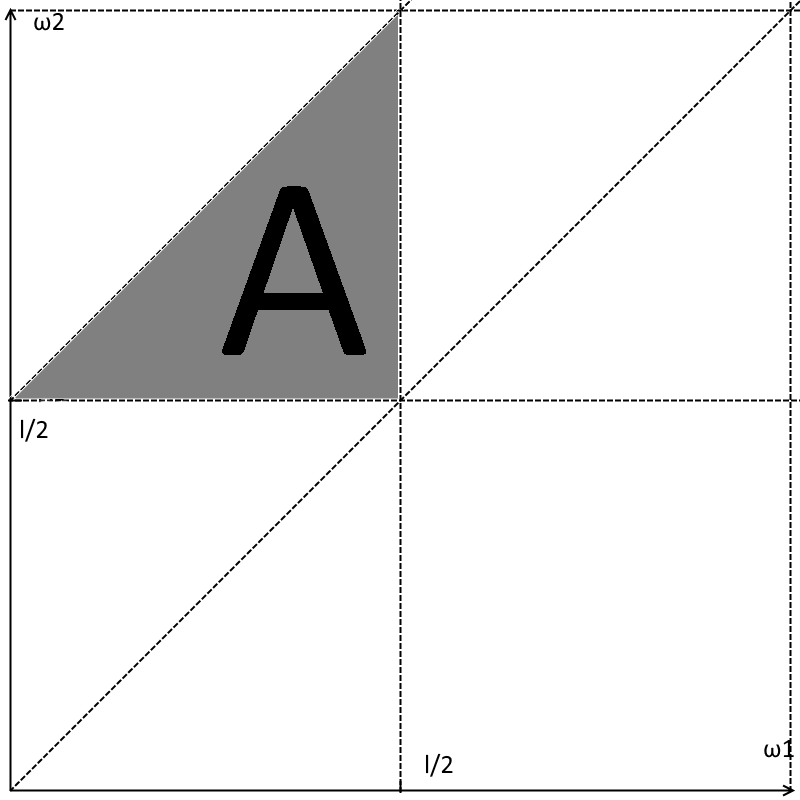
\includegraphics[width=100pt]{triangle.png}
		
		$P(A)=\frac{1}{4}$, from the picture.
	\end{myex}
	
	Here is a similar construction, based on the number $|\Omega|$ of elements in $\Omega$.
	
	\begin{myprop}{}{}
		Let $1\leq|\Omega|<\infty$, $\mathcal{F}=\mathcal{P}(A), P(A)=\frac{|A|}{|\Omega|}\;\forall A\in\mathcal{F}$. Then, $(\Omega, \mathcal{F}, P)$ is a finite probability space called a Laplace probability space.\\
		
		$P$ is discrete uniform distribution on $\Omega$.
		
		\begin{proof}
			Apply Prop. \ref{pr:prob} with $\mu(A)=|A|$ (counting measure).
		\end{proof}
	\end{myprop}
	
	\begin{myrem}{}{}
		For Laplace probability spaces, probability mass function on $\Omega$ is\\
		
		$f(\omega)=P(\{\omega\})=\frac{|\{\omega\}|}{|\Omega|}=\frac{1}{|\Omega|}\;\forall\omega\in\Omega$
		
		so the discrete uniform distribution assigns equal probability $\frac{1}{|\Omega|}$ to each $\omega\in\Omega$.
	\end{myrem}
	
	\begin{myex}{}{}
		\begin{enumerate}
			\item Determine probability of obtaining 1 or 5 when rolling a fair, 6-sided die.
			\begin{align*}
				\Omega&=\{1, ..., 6\}\\
				\mathcal{F}&=\mathcal{P}(\Omega)\\
				P(A)&=\frac{|A|}{|\Omega|}\;\forall A\in\Omega
			\end{align*}
			
			Let $A=$``rolling 1 or 5"$=\{1, 5\}$. Then, $P(A)=\frac{2}{6}=\frac{1}{3}$.
			\item Determine probability of obtaining a sum of 2 and 7 when rolling the die twice.
			\begin{align*}
				\Omega&=\begin{matrix}
				\{(1, 1), & \dots & (1, 6),\\
				& \ddots & \\
				(6, 1), & \dots & (6, 6)\}
				\end{matrix}\\
				\mathcal{F}&=\mathcal{P}(\Omega)\\
				P(A)&=\frac{|A|}{|\Omega|}\;\forall A\in\mathcal{F}
			\end{align*}
			
			So,\\
			
			$P($``sum is 2"$)=\frac{1}{36}$\\
			
			$P($``sum is 7"$)=\frac{6}{36}=\frac{1}{6}$\\
			\item Determine probability of obtaining at least one 6 when rolling 3 times.
			\begin{align*}
				\Omega&=\{(\omega_1, \omega_2, \omega_3) | \omega_i\in\{1, ..., 6\}\;\forall i\}\\
				\mathcal{F}&=\mathcal{P}(\Omega)\\
				P(A)&=\frac{|A|}{|\Omega|}\;\forall A\in\mathcal{F}
			\end{align*}
			
			So, $P($``at least one 6"$)=1-P($``no 6s"$)=1-(\frac{5}{6})^3=\frac{91}{216}$
		\end{enumerate}
	\end{myex}
	
	\newpage
	\section{Probability Counting Techniques}
	\subsection{Basic Rules}
	
	\begin{myprop}{}{}
		\begin{enumerate}
			\item If $A_1, ..., A_n$ are pointwise disjoint finite sets, then\\
			$|\bigcup_{i=1}^{n}A_i|=\sum_{i=1}^{n}|A_i|$ (addition rule).
			\item If $A_1, ..., A_n$ are finite sets, then\\
			$|\prod_{i=1}^{n}A_i|=\prod_{i=1}^{n}|A_i|$ (multiplication rule).
		\end{enumerate}
		
		\begin{proof}
			By induction.
		\end{proof}
	\end{myprop}
	
\end{document}
